\documentclass[11pt]{article}

\usepackage[margin=1in]{geometry}
\usepackage[T1]{fontenc}
\usepackage[utf8]{inputenc}
\usepackage{amsmath,amssymb}
\usepackage{booktabs}
\usepackage{graphicx}
\usepackage{microtype}
\usepackage{natbib}
\usepackage{hyperref}

\hypersetup{
  pdftitle={Residual Predictive Information in Prime Gaps},
  pdfauthor={Asger Othmar Fr\o hlich},
  pdfsubject={Prequential residual-coding protocol for consecutive prime gaps},
  pdfkeywords={prime gaps, prequential prediction, residual predictive information, arithmetic null models, universal coding, minimum description length},
  colorlinks=true,
  linkcolor=blue,
  citecolor=blue,
  urlcolor=blue
}

\title{Residual Predictive Information in Prime Gaps:\\
A Prequential Falsification Protocol and a Negative Result Beyond Wheel-First-Hit Baselines}
\author{Asger Othmar Fr{\o}hlich}
\date{June 30, 2026}

\newcommand{\Rgain}{R_k(X)}
\newcommand{\GX}{G_X}
\newcommand{\BX}{B_k}
\newcommand{\UX}{U_k}
\newcommand{\BOne}{B_1(11)}

\begin{document}
\maketitle

\begin{abstract}
Probabilistic models of the primes are useful not because the primes are random, but because they separate arithmetic structure that has been explicitly modeled from structure that remains unexplained. This paper studies that separation for consecutive prime gaps. For dyadic windows $[X,2X)$, let $G_X$ be the block of gaps beginning at primes $p_n\in[X,2X)$. Given an arithmetic online baseline $B_k$ and a penalized online residual predictor $U_k$, define the residual code gain
\[
R_k(X)=\frac{L_{B_k}(G_X)-L_{U_k}(G_X)}{|G_X|}.
\]
Positive $R_k(X)$ means that previous gap history improves prequential prediction after the declared arithmetic baseline has already been supplied.

The paper-scale experiments evaluate this protocol through $X=2^{26}$. The residual machinery detects a large signal against a deliberately weak local-density baseline $B_0$: a rank-mod-64 context-tree residual coder obtains $0.2674244536300398$ bits per gap, or about $974{,}961$ bits of total code gain at $X=2^{26}$. The same residual machinery gives null-level behavior once the wheel-first-hit baseline $B_1(11)$ is used. The main $B_1(11)$ bucket-residual test gives
\[
R=-2.7429243523407067\cdot10^{-7}
\]
bits per gap at $X=2^{26}$, with $z=-0.318$ against 200 stop-time synthetic null replicates and null 5--95\% interval
\[
[-2.7445474076652\cdot10^{-7},-2.7406420776259464\cdot10^{-7}].
\]
The conclusion is deliberately finite-scale and model-class-specific: under the tested residual predictors and through $X=2^{26}$, no positive residual predictive information is detected beyond the $B_1(11)$ wheel-first-hit baseline. The contribution is a reproducible prequential falsification protocol, a positive control showing that the residual coders are sensitive to omitted arithmetic structure, and a controlled negative result once that structure is included. The paper does not claim an asymptotic theorem and does not claim that prime gaps contain no residual information.
\end{abstract}

\section{Introduction}

The sequence of primes is deterministic. In an absolute sense, the primes are neither generated by independent randomness nor incompressible as a finite object: a short algorithm can generate them. Nevertheless, probabilistic models are central in the study of primes. Cram\'er-type models, random-sieve models, and Hardy--Littlewood tuple heuristics provide a language for distinguishing structure that is expected from local arithmetic constraints from structure that would remain surprising after those constraints have been built into the null model \citep{cramer1936,hardylittlewood1923,maier1985,montgomerysoundararajan2004,banksetal2023,lemkeoliver2016}.

This paper asks a relative and predictive question: after specified arithmetic structure has been built into an explicit online null model, does previous prime-gap history improve prediction of the next gap? This formulation is intentionally narrower than asking whether prime gaps are random or compressible. A residual learner should not receive credit for rediscovering arithmetic information that the baseline failed to encode. For example, a local-density model that ignores small-prime congruence constraints is too weak: a flexible residual model can detect the omitted wheel structure and obtain a large code gain. That gain is real relative to the weak baseline, but it is not evidence for residual sequential information beyond known arithmetic structure.

The question also differs from existing studies of prime-gap correlations, consecutive-prime biases, entropy-like statistics, or compression of prime-derived sequences \citep{lemkeoliver2016,kumar2003}. Those studies ask whether prime-derived data display structure relative to a chosen statistical summary or heuristic model. Here the target is operational and relative: before each gap is revealed, a declared arithmetic baseline has already assigned a probability distribution, and a residual learner receives credit only if previous gap history shortens the prequential code after that baseline and after its own complexity penalty. Thus the experiment is not an absolute randomness test for the primes. It is a test of residual online predictive gain after specified arithmetic information has been made explicit.

The protocol developed here measures residual predictive information by prequential code length \citep{dawid1984,barronrissanenyu1998,grunwald2019}. Before each gap is revealed, a baseline $B_k$ assigns an online probability distribution using declared arithmetic information. A residual predictor $U_k$ is allowed to use previous gap history and the same declared arithmetic information, but it must be online and penalized. The statistic is the per-gap code gain
\[
R_k(X)=\frac{L_{B_k}(G_X)-L_{U_k}(G_X)}{|G_X|}.
\]
Positive values indicate that past gaps improve prediction beyond the arithmetic baseline. Null-level or negative values indicate that no residual gain is detected after the residual model pays its own complexity cost.

The main empirical result is negative. The implemented residual models detect strong missing structure under $B_0$, but the signal disappears under the wheel-first-hit baseline $B_1(11)$. This is not a failure of the protocol. It is the intended falsification behavior: a residual-information test should be able to distinguish missing baseline structure from robust residual sequential information.

The paper makes four contributions. First, it formulates a prequential information-theoretic protocol for testing residual predictive information in prime gaps. Second, it states an explicit hierarchy of arithmetic baselines and an admissibility discipline intended to prevent hidden reconstruction of the prime sequence. Third, it demonstrates that the residual machinery is active by showing a strong positive control against the weak baseline $B_0$. Fourth, it reports a finite-scale negative result beyond $B_1(11)$: no positive residual predictive information is detected through $X=2^{26}$ under the tested residual coders.

The claim is intentionally narrow. The paper does not claim that prime gaps contain no residual information, that all possible higher-order arithmetic baselines have been exhausted, or that the finite-scale result proves an asymptotic theorem.

\section{Observation Protocol and Admissible Information}

Let
\[
p_1<p_2<p_3<\cdots
\]
be the primes and define consecutive gaps
\[
g_n=p_{n+1}-p_n.
\]
For a scale parameter $X$, define
\[
I_X=\{n:X\leq p_n<2X\}
\]
and the corresponding gap block
\[
G_X=(g_n)_{n\in I_X}.
\]
All reported code lengths in this paper are evaluated on such dyadic blocks.

An arithmetic baseline $B_k$ is an online predictive distribution. Before $g_n$ is revealed, it assigns a probability
\[
B_{k,n}(g\mid\mathcal F_{n,k})
\]
to each possible next gap $g$. The information field $\mathcal F_{n,k}$ contains only information available before $g_n$ is revealed, together with the arithmetic features declared at baseline level $k$. For each $n$, the baseline is normalized:
\[
\sum_g B_{k,n}(g\mid\mathcal F_{n,k})=1.
\]

For any online predictor $Q$, define the prequential code length
\[
L_Q(G_X)=\sum_{n\in I_X}-\log_2 Q_n(g_n\mid\mathcal F_{n,k}),
\]
and the mean code length per gap
\[
h_Q(X)=\frac{L_Q(G_X)}{|I_X|}.
\]
The prediction assigned to $g_n$ must be made before $g_n$ is observed.

Given a baseline $B_k$ and an admissible residual predictor $U_k$, define
\[
R_k(X)=\frac{L_{B_k}(G_X)-L_{U_k}(G_X)}{|I_X|}.
\]
The interpretation is direct. If $R_k(X)>0$, the residual predictor improves on the arithmetic baseline by $R_k(X)$ bits per gap. If $R_k(X)\approx0$, no residual predictive information is detected at the tested scale and model resolution. If $R_k(X)<0$, the residual predictor performs worse after model complexity is paid. The statistic is relative. It is not an entropy of the primes and not an absolute randomness test.

A residual predictor $U_k$ is admissible relative to $B_k$ if it may use the same declared arithmetic information as $B_k$, together with previous gap-derived symbols, but may not use future gaps, future primes, primality testing of candidate offsets in the target window, direct sieving outside the declared finite modulus set, or any table or compressed representation of the target block $G_X$.

A convenient sufficient form is
\[
U_k(g\mid\text{history},p_n)=U_s(s(g,p_n)\mid\text{history},p_n)B_k(g\mid p_n,s(g,p_n)),
\]
where $s(g,p_n)$ is a declared residual symbol and $B_k(g\mid p_n,s(g,p_n))$ is the baseline distribution conditional on that symbol. This allows the residual model to reweight declared symbols using past history without becoming a hidden prime generator.

The following table summarizes the intended information discipline.

\begin{table}[ht]
\centering
\small
\begin{tabular}{p{0.18\linewidth}p{0.38\linewidth}p{0.36\linewidth}}
\toprule
Component & Permitted information & Excluded information \\
\midrule
$B_0$ & Current scale and local density; parity/even-gap support & Small-prime wheel residues beyond parity; tuple corrections; future gaps \\
$B_1(11)$ & Current prime residue modulo $2310$, wheel-admissible offsets, local scale & Tuple corrections beyond the wheel; global analytic corrections; future gaps \\
Residual predictor $U_k$ & Same declared arithmetic information as $B_k$, previous gap-derived symbols, chronological training windows & Primality tests of $p_n+m$, hidden sieving of the test window, target-window tuning, future gaps \\
Synthetic nulls & Samples generated from the same declared baseline and evaluated by the same residual machinery & Conditioning choices not used for the real sequence unless explicitly declared \\
\bottomrule
\end{tabular}
\caption{Information discipline used to separate residual predictability from hidden reconstruction of the prime sequence.}
\label{tab:information-discipline}
\end{table}

This restriction is what makes the result interpretable. Without it, an apparently strong residual predictor could simply become a disguised prime generator.

\section{Arithmetic Null Models}

The null model is not a single universal object. The residual question only becomes meaningful relative to a declared arithmetic baseline. We use the hierarchy
\[
B_0\subset B_1\subset B_2\subset B_3\subset\cdots
\]
of progressively stronger baselines.

\subsection{Local-density baseline $B_0$}

The weakest baseline $B_0$ uses only the local density of primes near $p_n$. Since primes near $x$ have density approximately $1/\log x$, a simple even-gap model is
\[
B_0(g_n=2j\mid p_n)=(1-\theta_n)^{j-1}\theta_n,
\qquad
\theta_n\approx \frac{2}{\log p_n}.
\]
This baseline captures the scale of typical gaps but not small-prime divisibility constraints beyond parity. It is therefore expected to leave detectable arithmetic structure in the residual sequence. In this paper, $B_0$ is used mainly as a positive-control baseline.

\subsection{Wheel-first-hit baseline $B_1(y)$}

The wheel-corrected baseline $B_1(y)$ incorporates congruence constraints modulo the product of all primes up to a declared cutoff $y$:
\[
W_y=\prod_{q\leq y}q,
\qquad
\varphi_y=\varphi(W_y).
\]
Let
\[
\mathcal U_y=\{u\in\{0,1,\ldots,W_y-1\}:\gcd(u,W_y)=1\}
\]
be the reduced residue classes modulo $W_y$. For a current prime $p$, write $r=p\bmod W_y$. The one-period wheel-admissible offsets are the sorted values
\[
D_y(r)=\operatorname{sort}\{d(u,r):u\in\mathcal U_y\},
\]
where
\[
d(u,r)=
\begin{cases}
(u-r)\bmod W_y, & (u-r)\bmod W_y\neq0,\\
W_y, & (u-r)\bmod W_y=0.
\end{cases}
\]
Thus $D_y(r)\subseteq\{1,\ldots,W_y\}$ and $|D_y(r)|=\varphi_y$. An offset $m>0$ is admissible at $p$ if and only if
\[
\gcd(p+m,W_y)=1.
\]
Offsets failing this condition receive probability zero under $B_1(y)$.

For $m>0$, define the number of wheel-admissible offsets up to $m$ by
\[
C_y(p,m)=
\left\lfloor\frac{m}{W_y}\right\rfloor\varphi_y
+
\#\{d\in D_y(p\bmod W_y):d\leq m\bmod W_y\},
\]
with the convention that $C_y(p,m)=0$ for $m\leq0$. Equivalently, the $k$-th admissible offset is
\[
a_y(p,k)=
\left\lfloor\frac{k-1}{\varphi_y}\right\rfloor W_y
+d_{((k-1)\bmod\varphi_y)+1},
\]
where $d_1<\cdots<d_{\varphi_y}$ are the elements of $D_y(p\bmod W_y)$.

The baseline assumes a geometric first-hit law on this ordered admissible sequence. The conditional success probability among admissible positions is
\[
\theta_y(p)=\operatorname{clip}\left(\frac{W_y}{\varphi_y\log p},10^{-12},1-10^{-12}\right),
\]
where the clipping only prevents degenerate floating-point probabilities. For an admissible offset $m$, let $k_y(p,m)=C_y(p,m)$. The wheel-first-hit probability assigned to the exact next gap $g=m$ is
\[
B_{1,y}(g=m\mid p)=(1-\theta_y(p))^{k_y(p,m)-1}\theta_y(p),
\qquad \gcd(p+m,W_y)=1.
\]
For non-admissible offsets,
\[
B_{1,y}(g=m\mid p)=0,
\qquad \gcd(p+m,W_y)>1.
\]
The normalization follows from the geometric series over the ordered admissible offsets:
\[
\sum_{k=1}^{\infty}(1-\theta_y(p))^{k-1}\theta_y(p)=1.
\]
Thus $B_1(y)$ is a proper online distribution over positive offsets once the finite wheel and current prime $p$ have been declared.

The headline experiments use $B_1(11)$. In that case,
\[
W=2\cdot3\cdot5\cdot7\cdot11=2310,
\qquad
\varphi(W)=480.
\]
Therefore the model treats the next prime as the first success in the ordered sequence of offsets that are coprime to $2310$, using the local hit probability
\[
\theta_{11}(p)=\operatorname{clip}\left(\frac{2310}{480\log p},10^{-12},1-10^{-12}\right).
\]

For the bucket-residual experiment, the baseline exact-gap distribution also induces a bucket distribution. Let bucket edges be
\[
0=e_0<e_1<\cdots<e_J=\infty,
\]
and assign gap $g$ at prime $p$ to bucket $b$ when
\[
e_b\leq \frac{g}{\log p}<e_{b+1}.
\]
The corresponding baseline bucket mass is
\[
B_{1,y}^{\mathrm{bucket}}(b\mid p)=
\sum_{m:e_b\leq m/\log p<e_{b+1}} B_{1,y}(g=m\mid p).
\]
In the implementation this sum is evaluated by admissible-rank counts. If
\[
\ell_b(p)=\max\{1,\lceil e_b\log p\rceil\},
\qquad
\nu_b(p)=\lceil e_{b+1}\log p\rceil-1,
\]
then, for a finite upper edge,
\[
B_{1,y}^{\mathrm{bucket}}(b\mid p)=
(1-\theta_y(p))^{C_y(p,\ell_b(p)-1)}
\left[1-(1-\theta_y(p))^{C_y(p,\nu_b(p))-C_y(p,\ell_b(p)-1)}\right],
\]
with mass zero if $\nu_b(p)<\ell_b(p)$. For the final infinite bucket, the mass is
\[
(1-\theta_y(p))^{C_y(p,\ell_b(p)-1)}.
\]
These bucket masses partition unity and define the baseline expert used in the bucket-residual mixture.

\subsection{Why $B_1(11)$ is the main falsification threshold}

The role of $B_1(11)$ is deliberately limited but central. The $B_0$ model is a useful positive-control baseline precisely because it omits elementary small-modulus arithmetic. A residual learner that separates from $B_0$ may therefore be detecting omitted wheel structure rather than sequential information in prime gaps. The wheel-first-hit model supplies the finite congruence support up to $11$ and calibrates the first-hit law on the ordered admissible offsets. It is the first tested level at which the dominant small-prime obstruction has been made explicit.

For that reason, the paper's central falsification question is not whether every conceivable arithmetic correction has been exhausted. It is whether the residual signals found under a weak baseline remain after the elementary wheel obstruction has been supplied. They do not. This makes $B_1(11)$ a meaningful threshold for a negative methodological result, while preserving the narrower interpretation: the claim is beyond this explicit wheel-first-hit baseline and the tested residual predictors, not beyond all possible arithmetic null models.

\subsection{Higher-order baselines}

A natural $B_2$ baseline would incorporate finite tuple corrections. For a finite offset set
\[
\mathcal H=\{0,h_1,\ldots,h_s\},
\]
Hardy--Littlewood heuristics predict correction by the singular series \citep{hardylittlewood1923}
\[
\mathfrak S(\mathcal H)=
\prod_q
\left(1-\frac1q\right)^{-|\mathcal H|}
\left(1-\frac{\nu_q(\mathcal H)}q\right),
\]
where $\nu_q(\mathcal H)$ is the number of occupied residue classes modulo $q$.

The repository contains several $B_2$-style prototype diagnostics, including pair singular-series reweighting, residue-transition calibration, finite consecutive-prime inclusion-exclusion, and endpoint/exclusion shrinkage. These are useful diagnostics, but they are not treated as a canonical or exhaustive tuple-corrected hierarchy. The paper therefore does not claim that all $B_2$-level arithmetic structure has been ruled out.

A still stronger $B_3$-style baseline could incorporate predetermined global analytic corrections, such as smooth corrections from $\operatorname{Li}(x)$, explicit-formula terms using a bounded set of zeta zeros, or related global intensity corrections. No $B_3$-style correction is implemented in the paper-scale suite.

\section{Residual Predictors}

For each baseline $B_k$, the residual predictor $U_k$ is constructed so that it modifies only a declared residual symbolization while preserving the baseline's within-symbol distribution. This prevents the residual model from becoming a hidden replacement for the arithmetic baseline.

The general construction is
\[
U(g\mid \text{history},p)=
U_s(s(g,p)\mid\text{history},p)\,B(g\mid p,s(g,p)),
\]
where $s(g,p)$ is a declared residual symbol, $U_s$ is an online predictor for the symbol sequence, and $B(g\mid p,s(g,p))$ is the baseline distribution conditional on that symbol. Thus the residual model can reweight symbols using past history, but it cannot choose arbitrary exact gaps after observing the future.

Two residual families are used in the paper-scale suite.

\subsection{Bucket residual model}

The main $B_1(11)$ test uses buckets of the normalized gap
\[
\frac{g_n}{\log p_n}.
\]
The residual model is a Bayesian two-expert mixture between the baseline bucket distribution induced by $B_1(11)$ and a Krichevsky--Trofimov-smoothed finite-depth Markov predictor on previous buckets \citep{krichevskytrofimov1981,rissanen1984}. The mixture includes the baseline expert. Therefore, a positive residual gain requires the sequential bucket expert to improve prediction enough to overcome its own mixture cost. A null-level result is meaningful: the residual learner was given an opportunity to exploit bucket-level sequential dependence, but it did not improve beyond the baseline at the tested scale.

\subsection{Rank-mod-64 CTW residual model}

The positive-control residual model uses a rank symbol. Under the wheel-first-hit model, each admissible offset has a first-hit rank. The symbol is
\[
s(g,p)=\operatorname{rank}_{B_1}(g,p)\bmod 64.
\]
A sparse context-tree-weighting-style predictor is then applied to the symbol sequence \citep{willems1995}. The same residual machinery is evaluated against both $B_0$ and $B_1(11)$. This comparison is essential: a method that detects structure under $B_0$ but not under $B_1(11)$ supports the interpretation that the $B_0$ signal is omitted wheel structure rather than robust residual sequential information.

\section{Synthetic Nulls and Claim Criteria}

For each baseline, synthetic null sequences are generated from the same baseline and evaluated using the same residual machinery. The headline paper-scale runs use stop-time nulls: for each dyadic window, the synthetic process continues until it reaches the same endpoint scale rather than being forced to match the exact number of real gaps.

Stop-time nulls are preferable for the present question because the number of gaps in a window is itself part of the stochastic behavior induced by the baseline. Fixed-count nulls can be useful diagnostics, but the main significance comparison should not condition away endpoint behavior unless that conditioning is explicitly intended.

A positive residual-information claim would require all of the following: positive code gain beyond $B_1(11)$; survival against stop-time synthetic nulls; agreement across at least two independent residual symbolizations; absence, or substantial weakening, of the same effect in synthetic null sequences; persistence over increasing dyadic windows; and chronological tuning only. The completed paper-scale suite does not satisfy these criteria. The positive-control signal is strong under $B_0$, but it disappears under $B_1(11)$.

\begin{table}[ht]
\centering
\begin{tabular}{p{0.62\linewidth}p{0.28\linewidth}}
\toprule
Statement & Paper status \\
\midrule
The protocol detects omitted arithmetic structure under a weak local-density baseline. & Supported by the $B_0$ positive control. \\
Positive residual predictive information survives $B_1(11)$. & Not supported at $X\leq2^{26}$ by the tested residual predictors. \\
Prime gaps contain no residual information. & Not claimed. \\
The finite-scale result proves an asymptotic theorem. & Not claimed. \\
Implemented $B_2$-style diagnostics exhaust tuple-corrected arithmetic baselines. & Not claimed. \\
The contribution is a falsifiable empirical protocol plus a controlled negative result. & Main framing. \\
\bottomrule
\end{tabular}
\caption{Claim discipline for the paper.}
\label{tab:claim-discipline}
\end{table}

\section{Experiments and Reproducibility}

The paper-scale experiments use dyadic windows $X=2^m$ through $m=26$. The main runs use 200 synthetic null replicates/checkpoints, a common seed, chronological training windows, and checkpointed/resumable null generation.

The completed paper-scale suite consists of three experiment blocks. The first is the main $B_1(11)$ bucket-residual test, using buckets of $g/\log p$, a depth-4 finite-depth Markov bucket predictor in a baseline/residual mixture, stop-time nulls, and 200 null replicates. The second is the rank-mod-64 CTW control, evaluated under both $B_0$ and $B_1(11)$, using depth 1, stop-time nulls, and 200 null replicates. The third is the exact $B_0/B_1$ baseline ladder, comparing exact baseline code lengths under $B_0$ and $B_1(11)$.

The repository pins the paper-scale artifact record in a final manifest, derives the headline metrics from that record, regenerates a compact report, validates artifact completeness and metric consistency, audits cross-exponent robustness, and regenerates all manuscript figures. These checks are intended to make the empirical claim reproducible from committed artifacts without rerunning the long simulations.

Exact values are preserved in the machine-readable final metrics file; the manuscript rounds some displayed values for readability.

\section{Results}

\subsection{Main $B_1(11)$ bucket-residual result}

At $X=2^{26}=67{,}108{,}864$, the main $B_1(11)$ bucket-residual test contains $n=3{,}645{,}744$ gaps. The observed residual code gain is
\[
R=-2.7429243523407067\cdot10^{-7}
\]
bits per gap. The stop-time synthetic null distribution has mean
\[
-2.7425414055848714\cdot10^{-7},
\]
with 5--95\% interval
\[
[-2.7445474076652\cdot10^{-7},-2.7406420776259464\cdot10^{-7}].
\]
The observed value has $z=-0.31818465586295164$ against this null distribution. This is ordinary null-level behavior and gives no evidence for positive residual predictive information beyond $B_1(11)$.

\begin{figure}[ht]
\centering
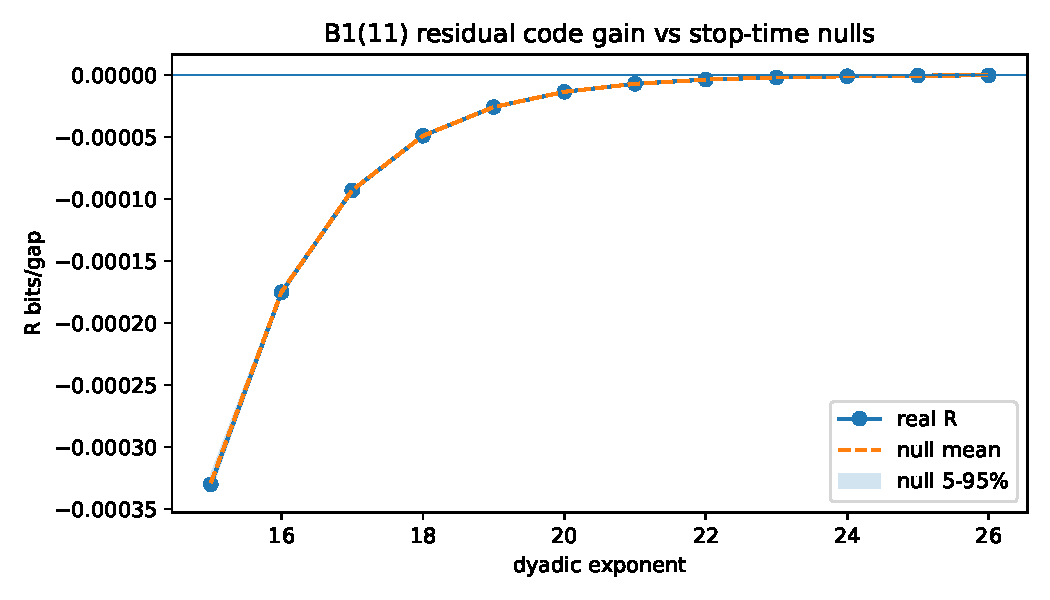
\includegraphics[width=0.82\linewidth]{paper_figures/figure_1_b1_residual_stop_time.pdf}
\caption{Main $B_1(11)$ bucket-residual result across dyadic exponents. The real residual gain remains inside the 5--95\% stop-time synthetic null band, including at $X=2^{26}$.}
\label{fig:b1-residual}
\end{figure}

\subsection{Positive control against $B_0$}

The rank-mod-64 CTW residual model gives a strong positive result against the weak $B_0$ baseline. At $X=2^{26}$,
\[
R=0.2674244536300398
\]
bits per gap, corresponding to total code gain
\[
974{,}961.0972749958
\]
bits. The empirical upper-tail $p$-value is
\[
p_{\geq}=0.004975124378109453.
\]
This confirms that the residual machinery is active: it can detect missing structure when the arithmetic baseline is too weak.

Under $B_1(11)$, the same rank-mod-64 CTW residual model gives
\[
R=-2.742924352340597\cdot10^{-7}
\]
bits per gap, corresponding to approximately $-1$ bit of total gain. The empirical upper-tail $p$-value is $p_{\geq}=0.6119402985074627$. Thus, the same residual machinery that strongly separates from the $B_0$ null gives null-level behavior under $B_1(11)$. This is the central empirical pattern of the paper.

\begin{figure}[ht]
\centering
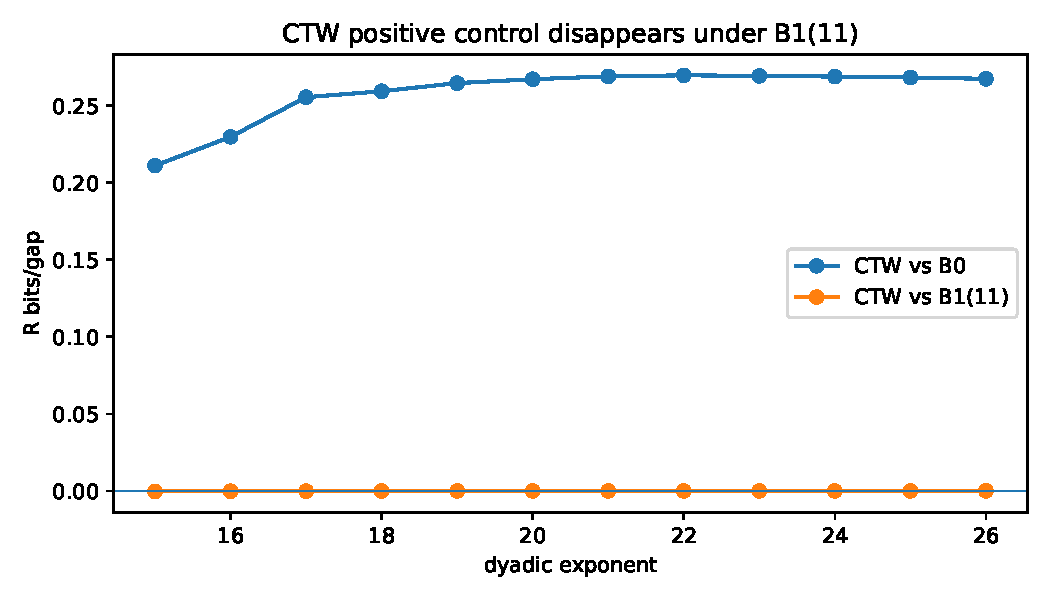
\includegraphics[width=0.82\linewidth]{paper_figures/figure_2_ctw_positive_control.pdf}
\caption{Rank-mod-64 CTW control. The residual coder strongly separates from the weak $B_0$ baseline, but the same residual machinery is null-level under $B_1(11)$. The $B_1(11)$ curve is visually indistinguishable from zero on the $B_0$ scale; the exact endpoint value is reported in Table~\ref{tab:headline-results}.}
\label{fig:ctw-control}
\end{figure}

\subsection{Exact baseline ladder}

At $X=2^{26}$, the exact baseline code lengths are
\[
B_0=4.563439906212204
\]
bits per gap and
\[
B_1(11)=3.1704284777012335
\]
bits per gap. The improvement of $B_1(11)$ over $B_0$ is therefore
\[
1.3930114285109703
\]
bits per gap. This improvement is large compared with the residual effects being tested after $B_1(11)$. It explains why a weak baseline can generate apparent residual structure: much of that structure is small-modulus arithmetic information not yet included in the null.

\begin{figure}[ht]
\centering
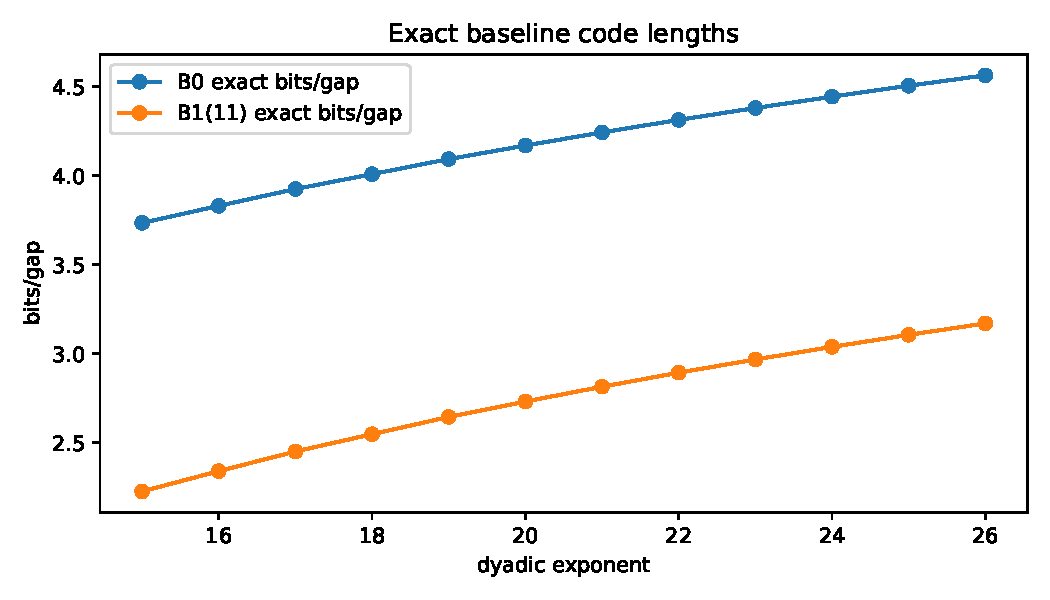
\includegraphics[width=0.82\linewidth]{paper_figures/figure_3_baseline_ladder_bits.pdf}
\caption{Exact baseline ladder. The wheel-first-hit baseline $B_1(11)$ substantially improves code length relative to the weak local-density baseline $B_0$ across the tested range.}
\label{fig:baseline-ladder}
\end{figure}

\begin{table}[ht]
\centering
\small
\begin{tabular}{p{0.36\linewidth}p{0.30\linewidth}p{0.24\linewidth}}
\toprule
Quantity at $X=2^{26}$ & Value & Interpretation \\
\midrule
Main $B_1(11)$ bucket residual & $-2.7429\cdot10^{-7}$ bits/gap & Null-level \\
Main $B_1(11)$ null 5--95\% interval & $[-2.7445,-2.7406]\cdot10^{-7}$ & Real value inside band \\
Rank-mod-64 CTW under $B_0$ & $0.2674$ bits/gap & Strong positive control \\
Rank-mod-64 CTW under $B_1(11)$ & $-2.7429\cdot10^{-7}$ bits/gap & Null-level \\
Exact $B_0$ code length & $4.5634$ bits/gap & Weak baseline \\
Exact $B_1(11)$ code length & $3.1704$ bits/gap & Wheel baseline \\
$B_0-B_1(11)$ improvement & $1.3930$ bits/gap & Wheel structure absorbed \\
\bottomrule
\end{tabular}
\caption{Headline paper-scale metrics at $X=2^{26}$. Values are rounded for readability; exact values are stored in \texttt{experiments/final\_metrics.json}.}
\label{tab:headline-results}
\end{table}

\subsection{Cross-exponent robustness}

The negative $B_1(11)$ result is not only an endpoint observation. Across the tested dyadic exponents, the main $B_1(11)$ bucket residual remains inside the 5--95\% stop-time null band and has small absolute $z$-scores. The rank-mod-64 CTW positive control separates from $B_0$ across tested exponents, while the same residual model remains null-consistent under $B_1(11)$. The baseline ladder also keeps $B_1(11)$ below $B_0$ across the tested range.

These checks support the qualitative conclusion: the protocol detects missing structure under weak baselines, but does not detect positive residual predictive information beyond the implemented wheel-first-hit baseline.

\section{Discussion}

The main lesson is methodological. Patterns in prime gaps are easy to find. A pattern should count as residual predictive information only if it survives an explicit arithmetic null model, an online prediction rule, and a complexity penalty.

The $B_0$ result shows that residual learners can produce large apparent gains when the baseline omits known arithmetic structure. The $B_1(11)$ result shows that this gain disappears after small-modulus wheel structure is included. This supports the interpretation that the detected $B_0$ signal is arithmetic baseline structure, not robust residual sequential information.

The negative result is informative because the protocol contains its own positive control. A residual test that never detects anything would be unconvincing; a residual test that detects structure under a weak baseline but loses that signal under a stronger arithmetic null is more credible. The comparison shows that the residual machinery is sensitive, but also that the main positive signal is not stable under a fairer baseline.

Several reviewer objections are therefore addressed by design rather than by rhetoric. If the concern is that the residual models are too weak to find any signal, the $B_0$ positive control shows that they can find omitted arithmetic structure. If the concern is that the negative result is merely an endpoint accident, the cross-exponent audit checks the same qualitative pattern across dyadic windows. If the concern is that $B_1(11)$ is not a complete model of prime gaps, that concern is accepted: the claim is deliberately only beyond this declared wheel-first-hit baseline and the tested residual predictors, not beyond all arithmetic null models.

The result also clarifies the role of higher-order baselines. A stronger $B_2$ or $B_3$ model may absorb additional structure, and future work should develop such baselines more canonically. The present paper does not need to exhaust those levels to support its narrow claim. The claim is limited to the tested residual predictors beyond $B_1(11)$: at the tested scale, the first level at which small-prime wheel structure is included is sufficient to eliminate the residual signals tested here.

This framing is deliberately conservative. A future residual model could still obtain positive code gain beyond $B_1(11)$, and a future arithmetic hierarchy could change what is counted as residual. The contribution here is the measurement protocol and the observed falsification of the tested residual signal, not a final theory of prime-gap predictability.

\section{Limitations and Threats to Validity}

The limitations are substantial and define the scope of the paper. First, the result is finite-scale. The largest endpoint is $X=2^{26}$, not an asymptotic regime. The paper should therefore be read as an empirical falsification study at a reproducible scale.

Second, the negative result is model-class-specific. It applies to the tested bucket residual model and rank-mod-64 CTW residual model. It does not exclude all possible residual predictors.

Third, $B_1(11)$ is not a complete arithmetic model of prime gaps. It incorporates finite wheel constraints up to $11$, but it does not incorporate a canonical tuple-corrected $B_2$ hierarchy or global analytic corrections.

Fourth, the implemented $B_2$-style diagnostics are not exhaustive. They should be treated only as auxiliary checks. They should not be described as ruling out tuple-corrected arithmetic structure in general.

Fifth, the number of synthetic null replicates is 200. This is adequate for a first finite-scale negative study and for detecting gross departures from the null, but it is not designed to support extremely small $p$-value claims.

Sixth, the implementation is a research implementation. The repository includes artifact validation, pinned metrics, figure regeneration, and a robustness audit, but further independent replication and unit testing would strengthen confidence in the result.

These limitations are not incidental. They are part of the claim discipline. The contribution is a protocol and a controlled finite-scale result, not a final theory of prime-gap predictability.

\section{Code and Data Availability}

The code, manuscript sources, pinned paper-scale artifacts, generated figures, validation scripts, final metrics, and reproducibility workflows are available in the repository \url{https://github.com/asgerof/residual-predictive-information-of-prime-gaps}. Archived releases are available through Zenodo; for exact reproducibility, cite the version-specific DOI shown on Zenodo for the GitHub release used.

The reported numbers are pinned by the final manifest, and the compact report is regenerated from that manifest. The validation and robustness-audit scripts check artifact completeness, metric consistency, and the cross-exponent qualitative conclusion. Long simulations are not rerun by default; the committed artifacts are the reproducible paper-scale record.

\section{Conclusion}

This paper introduced a prequential residual-coding protocol for measuring predictive information in consecutive prime gaps relative to explicit arithmetic null models. The central statistic is
\[
R_k(X)=\frac{L_{B_k}(G_X)-L_{U_k}(G_X)}{|G_X|}.
\]
The protocol distinguishes residual predictability from omitted baseline structure. Against a weak $B_0$ baseline, the rank-mod-64 CTW residual model obtains a large positive code gain. Against the wheel-first-hit baseline $B_1(11)$, the same residual machinery gives null-level behavior. The main $B_1(11)$ bucket-residual test also gives null-level behavior through $X=2^{26}$.

The safest conclusion is finite-scale and model-class-specific: under the tested online residual predictors and through $X=2^{26}$, no positive residual predictive information is detected beyond the $B_1(11)$ wheel-first-hit baseline.

This does not prove that prime gaps contain no residual information. It shows that a controlled residual-coding protocol can separate weak-baseline artifacts from robust residual signals, and that the tested positive signal disappears once small-prime wheel structure is included.

\bibliographystyle{plainnat}
\bibliography{references}

\end{document}
